% !Mode:: "TeX:UTF-8"

\def\usewhat{pdflatex}                               % 定义编译方式 dvipdfmx 或者 pdflatex,默认为 dvipdfmx
                                                     % 方式编译,如果需要修改,只需改变花括号中的内容即可。
\documentclass[12pt,openany,oneside,ctexartutf8]{book}
                                                     % 本科生毕业论文通常采用单页排版
% !Mode:: "TeX:UTF-8"
%  Authors: 张井   Jing Zhang: prayever@gmail.com     天津大学2010级管理与经济学部信息管理与信息系统专业硕士生
%           余蓝涛 Lantao Yu: lantaoyu1991@gmail.com  天津大学2008级精密仪器与光电子工程学院测控技术与仪器专业本科生

%%%%%%%%%% Package %%%%%%%%%%%%
\usepackage{graphicx}                       % 支持插图处理
% \usepackage[a4paper,text={146.4true mm,239.2 true mm},top= 25.4true mm, bottom= 25.4true mm, left=31.7 true mm,head=6true mm,headsep=6.5true mm,foot=16.5true mm]{geometry}
\usepackage[a4paper,top=25.4mm, bottom=25.4mm, left=31.7mm, right=31.7mm, head=6true mm,headsep=6.5true mm,foot=17.5mm]{geometry}
                                            % 支持版面尺寸设置
\usepackage[squaren]{SIunits}               % 支持国际标准单位

\usepackage{titlesec}                       % 控制标题的宏包
\usepackage{titletoc}                       % 控制目录的宏包
\usepackage{fancyhdr}                       % fancyhdr宏包 支持页眉和页脚的相关定义
\usepackage[UTF8]{ctex}                     % 支持中文显示
\usepackage{CJKpunct}
\usepackage{color}                          % 支持彩色
\usepackage{amsmath}                        % AMSLaTeX宏包 用来排出更加漂亮的公式
\usepackage{amssymb}                        % 数学符号生成命令
\usepackage[below]{placeins}    %允许上一个section的浮动图形出现在下一个section的开始部分,还提供\FloatBarrier命令,使所有未处理的浮动图形立即被处理
\usepackage{multirow}                       % 使用Multirow宏包,使得表格可以合并多个row格
\usepackage{booktabs}                       % 表格,横的粗线;\specialrule{1pt}{0pt}{0pt}
\usepackage{longtable}                      % 支持跨页的表格。
\usepackage{tabularx}                       % 自动设置表格的列宽
\usepackage{subfigure}                      % 支持子图 %centerlast 设置最后一行是否居中
\usepackage[subfigure]{ccaption}            % 支持子图的中文标题
\usepackage[sort&compress,numbers]{natbib}  % 支持引用缩写的宏包
\usepackage{enumitem}                       % 使用enumitem宏包,改变列表项的格式
\usepackage{calc}                           % 长度可以用+ - * / 进行计算
\usepackage{txfonts}                        % 字体宏包
\usepackage{bm}                             % 处理数学公式中的黑斜体的宏包
\usepackage[amsmath,thmmarks,hyperref]{ntheorem}  % 定理类环境宏包,其中 amsmath 选项用来兼容 AMS LaTeX 的宏包
\usepackage{CJKnumb}                        % 提供将阿拉伯数字转换成中文数字的命令
\usepackage{indentfirst}                    % 首行缩进宏包
\usepackage{CJKutf8}                        % 用在UTF8编码环境下,它可以自动调用CJK,同时针对UTF8编码作了设置

% \usepackage{fancybox} 

%\usepackage{hypbmsec}                      % 用来控制书签中标题显示内容
\newcommand{\tabincell}[2]{\begin{tabular}{@{}#1@{}}#2\end{tabular}}
\usepackage{xcolor}
%支持代码环境
\usepackage{listings}
\lstset{numbers=left,
language=[ANSI]{C},
numberstyle=\tiny,
extendedchars=false,
showstringspaces=false,
breakatwhitespace=false,
breaklines=true,
captionpos=b,
keywordstyle=\color{blue!70},
commentstyle=\color{red!50!green!50!blue!50},
frame=shadowbox,
rulesepcolor=\color{red!20!green!20!blue!20}
}
%支持算法环境
\usepackage[boxed,ruled,lined]{algorithm2e}
\usepackage{algorithmic}

\usepackage{array}
\newcommand{\PreserveBackslash}[1]{\let\temp=\\#1\let\\=\temp}
\newcolumntype{C}[1]{>{\PreserveBackslash\centering}p{#1}}
\newcolumntype{R}[1]{>{\PreserveBackslash\raggedleft}p{#1}}
\newcolumntype{L}[1]{>{\PreserveBackslash\raggedright}p{#1}}

% 生成有书签的 pdf 及其生成方式。通常可以在 tjumain.tex 文件的第一行选择 pdflatex 或者是 dvipdfmx 编译手段。如果选择前者,则使用 pdflatex + pdflatex 编译; 如果选择后者,在编译的时候选择 latex + bibtex + latex + latex 编译。出现混淆的时候,系统会报错。
% 如果您的pdf制作中文书签有乱码使用如下命令,就可以解决了
\def\atemp{pdflatex}\ifx\atemp\usewhat
\usepackage{cmap}                           % pdflatex 编译时,可以生成可复制、粘贴的中文 PDF 文档, 缺点是在Windows上显示时效果不大好,字体发虚
\usepackage{hyperref}
\hypersetup{
    unicode,
    pdfborder={0 0 0},
}
\fi
% \usepackage[pdftex,unicode,
%             CJKbookmarks=true,
%             bookmarksnumbered=true,
%             bookmarksopen=true,
%             colorlinks=false,
%             pdfborder={0 0 0},
%             citecolor=blue,
%             linkcolor=red,
%             anchorcolor=green,
%             urlcolor=blue,
%             breaklinks=true
%             ]{hyperref}

                                % 定义本文所使用宏包
\graphicspath{{figures/}}                            % 定义所有的 .eps 文件在 figures 子目录下
\begin{document}                                     % 开始全文
\begin{CJK*}{UTF8}{song}                             % 开始中文字体使用
	% !Mode:: "TeX:UTF-8"
%  Authors: 张井   Jing Zhang: prayever@gmail.com     天津大学2010级管理与经济学部信息管理与信息系统专业硕士生
%           余蓝涛 Lantao Yu: lantaoyu1991@gmail.com  天津大学2008级精密仪器与光电子工程学院测控技术与仪器专业本科生

% 2018/5/23修正
%           李幼萌 Youmeng Li: liyoumeng@tju.edu.cn   天津大学软件学院软件工程系

%%%%%%%%%%%%%%%%% Fonts Definition and Basics %%%%%%%%%%%%%%%%%
\newcommand{\song}{\CJKfamily{song}}    % 宋体
\newcommand{\fs}{\CJKfamily{fs}}        % 仿宋体
\newcommand{\kai}{\CJKfamily{kai}}      % 楷体
\newcommand{\hei}{\CJKfamily{hei}}      % 黑体
\newcommand{\li}{\CJKfamily{li}}        % 隶书
\newcommand{\yihao}{\fontsize{26pt}{26pt}\selectfont}       % 一号, 单倍行距
\newcommand{\xiaoyi}{\fontsize{24pt}{24pt}\selectfont}      % 小一, 单倍行距
\newcommand{\erhao}{\fontsize{22pt}{1.25\baselineskip}\selectfont}       % 二号, 1.25倍行距
\newcommand{\xiaoer}{\fontsize{18pt}{18pt}\selectfont}      % 小二, 单倍行距
\newcommand{\sanhao}{\fontsize{16pt}{16pt}\selectfont}      % 三号, 单倍行距
\newcommand{\xiaosan}{\fontsize{15pt}{15pt}\selectfont}     % 小三, 单倍行距
\newcommand{\sihao}{\fontsize{14pt}{14pt}\selectfont}       % 四号, 单倍行距
\newcommand{\xiaosi}{\fontsize{12pt}{12pt}\selectfont}      % 小四, 单倍行距
\newcommand{\wuhao}{\fontsize{10.5pt}{10.5pt}\selectfont}   % 五号, 单倍行距
\newcommand{\xiaowu}{\fontsize{9pt}{9pt}\selectfont}        % 小五, 单倍行距

\CJKtilde  % 重新定义了波浪符~的意义
\newcommand\prechaptername{第}
\newcommand\postchaptername{章}

\punctstyle{hangmobanjiao}             % 调整中文字符的表示,行内占一个字符宽度,行尾占半个字符宽度

% 调整罗列环境的布局
\setitemize{leftmargin=3em,itemsep=0em,partopsep=0em,parsep=0em,topsep=-0em}
\setenumerate{leftmargin=3em,itemsep=0em,partopsep=0em,parsep=0em,topsep=0em}

% 避免宏包 hyperref 和 arydshln 不兼容带来的目录链接失效的问题。
\def\temp{\relax}
\let\temp\addcontentsline
\gdef\addcontentsline{\phantomsection\temp}

% 自定义项目列表标签及格式 \begin{publist} 列表项 \end{publist}
\newcounter{pubctr} %自定义新计数器
\newenvironment{publist}{%%%%%定义新环境
\begin{list}{[\arabic{pubctr}]} %%标签格式
    {
     \usecounter{pubctr}
     \setlength{\leftmargin}{2.5em}   % 左边界 \leftmargin =\itemindent + \labelwidth + \labelsep
     \setlength{\itemindent}{0em}     % 标号缩进量
     \setlength{\labelsep}{1em}       % 标号和列表项之间的距离,默认0.5em
     \setlength{\rightmargin}{0em}    % 右边界
     \setlength{\topsep}{0ex}         % 列表到上下文的垂直距离
     \setlength{\parsep}{0ex}         % 段落间距
     \setlength{\itemsep}{0ex}        % 标签间距
     \setlength{\listparindent}{0pt}  % 段落缩进量
    }}
{\end{list}}

\makeatletter
\renewcommand\normalsize{
  \@setfontsize\normalsize{12pt}{12pt} % 小四对应 12 pt
  \setlength\abovedisplayskip{4pt}
  \setlength\abovedisplayshortskip{4pt}
  \setlength\belowdisplayskip{\abovedisplayskip}
  \setlength\belowdisplayshortskip{\abovedisplayshortskip}
  \let\@listi\@listI}
\def\defaultfont{\renewcommand{\baselinestretch}{1.63}\normalsize\selectfont} % 设置行距

\renewcommand{\CJKglue}{\hskip -0.1 pt plus 0.08\baselineskip} % 控制字间距,使每行 34 个汉字
\makeatother

%%%%%%%%%%%%% Contents %%%%%%%%%%%%%%%%%
\renewcommand{\contentsname}{目\qquad 录}
\setcounter{tocdepth}{1} % 控制目录深度
\titlecontents{chapter}[2em]{\vspace{.5\baselineskip}\xiaosan\song}
             {\prechaptername\CJKnumber{\thecontentslabel}\postchaptername\qquad}{}
             {\hspace{.5em}\titlerule*[10pt]{$\cdot$}\sihao\contentspage}
\titlecontents{section}[4.2em]{\vspace{.25\baselineskip}\sihao\song}
             {\thecontentslabel\quad}{}
             {\hspace{.5em}\titlerule*[10pt]{$\cdot$}\sihao\contentspage}
% \titlecontents{subsection}[4em]{\vspace{.25\baselineskip}\xiaosi\song}
%              {\thecontentslabel\quad}{}
%              {\hspace{.5em}\titlerule*[10pt]{$\cdot$}\sihao\contentspage}

%%%%%%%%%% Chapter and Section %%%%%%%%%%%%%
\setcounter{secnumdepth}{4}
\setlength{\parindent}{2em}

\renewcommand{\chaptername}{\prechaptername\CJKnumber{\thechapter}\postchaptername}
\titleformat{\chapter}{\centering}{\xiaosan\song}{\chaptername}{} %{2em}
\titlespacing{\chapter}{0pt}{0.1\baselineskip}{0.8\baselineskip}

\titleformat{\section}{\sihao\hei}{\thesection}{1em}{}
\titlespacing{\section}{0pt}{0.15\baselineskip}{0.25\baselineskip}

\titleformat{\subsection}{\sihao\hei}{\thesubsection}{1em}{}
\titlespacing{\subsection}{0pt}{0.1\baselineskip}{0.3\baselineskip}

\titleformat{\subsubsection}{\sihao\hei}{\thesubsubsection}{1em}{}
\titlespacing{\subsubsection}{0pt}{0.05\baselineskip}{0.1\baselineskip}

%%%%%%%%%% Table, Figure and Equation %%%%%%%%%%%%%%%%%
\renewcommand{\tablename}{表}                                     % 插表题头
\renewcommand{\figurename}{图}                                    % 插图题头
\renewcommand{\thefigure}{\arabic{chapter}-\arabic{figure}}       % 使图编号为 7-1 的格式 %\protect{~}
\renewcommand{\thesubfigure}{\alph{subfigure})}                   % 使子图编号为 a) 的格式
\renewcommand{\thesubtable}{(\alph{subtable})}                    % 使子表编号为 (a) 的格式
\renewcommand{\thetable}{\arabic{chapter}-\arabic{table}}         % 使表编号为 7-1 的格式
\renewcommand{\theequation}{\arabic{chapter}-\arabic{equation}}   % 使公式编号为 7-1 的格式

%%%%%% 定制浮动图形和表格标题样式 %%%%%%
\makeatletter
\long\def\@makecaption#1#2{
   \vskip\abovecaptionskip
   \sbox\@tempboxa{\centering\wuhao\song{#1\qquad #2} }
   \ifdim \wd\@tempboxa >\hsize
     \centering\wuhao\song{#1\qquad #2} \par
   \else
     \global \@minipagefalse
     \hb@xt@\hsize{\hfil\box\@tempboxa\hfil}
   \fi
   \vskip\belowcaptionskip}
\makeatother
\captiondelim{~~~~} %用来控制longtable表头分隔符

%%%%%%%%%% Theorem Environment %%%%%%%%%%%%%%%%%
\theoremstyle{plain}
\theorembodyfont{\song\rmfamily}
\theoremheaderfont{\hei\rmfamily}
\newtheorem{theorem}{定理~}[chapter]
\newtheorem{lemma}{引理~}[chapter]
\newtheorem{axiom}{公理~}[chapter]
\newtheorem{proposition}{命题~}[chapter]
\newtheorem{prop}{性质~}[chapter]
\newtheorem{corollary}{推论~}[chapter]
\newtheorem{definition}{定义~}[chapter]
\newtheorem{conjecture}{猜想~}[chapter]
\newtheorem{example}{例~}[chapter]
\newtheorem{remark}{注~}[chapter]
%\newtheorem{algorithm}{算法~}[chapter]
\newenvironment{proof}{\noindent{\hei 证明:}}{\hfill $ \square $ \vskip 4mm}
\theoremsymbol{$\square$}

%%%%%%%%%% Page: number, header and footer  %%%%%%%%%%%%%%%%%

%\frontmatter 或 \pagenumbering{roman}
%\mainmatter 或 \pagenumbering{arabic}
\makeatletter
\renewcommand\frontmatter{\clearpage
  \@mainmatterfalse
  }
\makeatother

%%%%%%%%%%%% References %%%%%%%%%%%%%%%%%
\renewcommand{\bibname}{参考文献}
% 重定义参考文献样式,来自thu
\makeatletter
\renewenvironment{thebibliography}[1]{
    \titleformat{\chapter}{\raggedright\sihao\hei}{\chaptername}{2em}{}
   \chapter*{\bibname}
   \wuhao
   \list{\@biblabel{\@arabic\c@enumiv}}
        {\renewcommand{\makelabel}[1]{##1\hfill}
         \settowidth\labelwidth{0 cm}
         \setlength{\labelsep}{0pt}
         \setlength{\itemindent}{0pt}
         \setlength{\leftmargin}{\labelwidth+\labelsep}
         \addtolength{\itemsep}{-0.7em}
         \usecounter{enumiv}
         \let\p@enumiv\@empty
         \renewcommand\theenumiv{\@arabic\c@enumiv}}
    \sloppy\frenchspacing
    \clubpenalty4000
    \@clubpenalty \clubpenalty
    \widowpenalty4000
    \interlinepenalty4000
    \sfcode`\.\@m}
   {\def\@noitemerr
     {\@latex@warning{Empty `thebibliography' environment}}
    \endlist\frenchspacing}
\makeatother

\addtolength{\bibsep}{-0.5em}     % 缩小参考文献间的垂直间距
\setlength{\bibhang}{2em}         % 每个条目自第二行起缩进的距离

% 参考文献引用作为上标出现
%\newcommand{\citeup}[1]{\textsuperscript{\cite{#1}}}
\makeatletter
    \def\@cite#1#2{\textsuperscript{[{#1\if@tempswa , #2\fi}]}}
\makeatother
%% 引用格式
\bibpunct{[}{]}{,}{s}{}{,}

%%%%%%%%%%%% Cover %%%%%%%%%%%%%%%%%
% 封面、摘要、版权、致谢格式定义
\makeatletter
\def\ctitle#1{\def\@ctitle{#1}}\def\@ctitle{}
\def\cdegree#1{\def\@cdegree{#1}}\def\@cdegree{}
\def\caffil#1{\def\@caffil{#1}}\def\@caffil{}
\def\csubject#1{\def\@csubject{#1}}\def\@csubject{}
\def\cgrade#1{\def\@cgrade{#1}}\def\@cgrade{}
\def\cauthor#1{\def\@cauthor{#1}}\def\@cauthor{}
\def\cnumber#1{\def\@cnumber{#1}}\def\@cnumber{}
\def\cstuid#1{\def\@cstuid{#1}}\def\@cstuid{}
\def\cdate#1{\def\@cdate{#1}}\def\@cdate{}
\long\def\cabstract#1{\long\def\@cabstract{#1}}\long\def\@cabstract{}
\long\def\eabstract#1{\long\def\@eabstract{#1}}\long\def\@eabstract{}
\def\ckeywords#1{\def\@ckeywords{#1}}\def\@ckeywords{}
\def\ekeywords#1{\def\@ekeywords{#1}}\def\@ekeywords{}
\def\cheading#1{\def\@cheading{#1}}\def\@cheading{}
\def\ccovertitle#1{\def\@ccovertitle{#1}}\def\@ccovertitle{}

\pagestyle{fancy}
  \fancyhf{}
  \fancyhead[C]{\song\wuhao \@cheading}  % 页眉显示天津大学 20XX 届本科生毕业论文
  \fancyfoot[C]{\song\xiaowu ~\thepage~}
\newlength{\@title@width}

% 定义封面
\def\makecover{
%\cleardoublepage%
   \phantomsection
    \pdfbookmark[-1]{\@ctitle}{ctitle}

    \begin{titlepage}
      \vspace*{10pt}
      \begin{center}

      \begin{figure}[h]
      \centering
      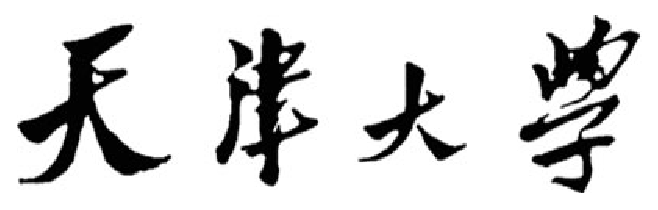
\includegraphics[width=0.4\textwidth]{figures/tju}
      \end{figure}
      \vspace*{15pt}
      \hei\erhao{\textbf{\@ccovertitle}} \\
      \hei\erhao{\textbf{\@ctitle}}
      \vspace*{55pt}

      \begin{figure}[h]
      \centering
      
\includegraphics[width=0.3\textwidth]{figures/Tjulogo}
      \end{figure}

      \vspace*{60pt}
      \renewcommand\arraystretch{1.5}
      \setlength{\@title@width}{8.5cm}
      {
        \sanhao\song{
          \begin{tabular}{lc}
            \textbf{学\qquad 院}  &  \underline{\makebox[\@title@width][c]{\textbf{\@caffil}}} \\
            \textbf{专\qquad 业}  &  \underline{\makebox[\@title@width][c]{\textbf{\@csubject}}} \\
            \textbf{年\qquad 级}  &  \underline{\makebox[\@title@width][c]{\textbf{\@cgrade}}}\\
            \textbf{姓\qquad 名}  &  \underline{\makebox[\@title@width][c]{\textbf{\@cauthor}}}\\
            \textbf{学\qquad 号}  &  \underline{\makebox[\@title@width][c]{\textbf{\@cstuid}}}\\
          \end{tabular}
        }
    }
    \vspace*{40pt}

    \song\sanhao{\textbf{\@cdate}}
    \end{center}
    \end{titlepage}
}

                             % 完成对论文各个部分格式的设置
	% !Mode:: "TeX:UTF-8"


%%%%%%%%%%%%%%%%%%%%%%%%%%%%%%%%%%%%%%%%%%%%%%%%%%%%%%%%%%%%%%%
%%  可通过对 setup/format.tex中                               %%
%%  第243行 \setlength{\@title@width}{5cm}中 5cm 这个参数来   %%
%%  控制封面中下划线的长度。                                   %%
%%%%%%%%%%%%%%%%%%%%%%%%%%%%%%%%%%%%%%%%%%%%%%%%%%%%%%%%%%%%%%

\cheading{天津大学软件学院~\the\year~年《软件工程综合实践》饿了么报告}      % 正文页眉
\ccovertitle{《软件工程综合实践》结课报告}                       % 封面标题

%%%%%%%%%%%%%%%%%%%%%%%%%%%%%%%%%%%%%%%%%%%%%%%%%%%%%%%%%%%%%
%%%%%%%%%% 以下为论文的基本信息,需要由作者进行修改 %%%%%%%%%%%%
%%%%%%%%%%%%%%%%%%%%%%%%%%%%%%%%%%%%%%%%%%%%%%%%%%%%%%%%%%%%%
\ctitle{~\LaTeX~模板使用说明}    % 封面用论文标题,自己可手动断行
\caffil{智能与计算}       % 学院名称
\csubject{软件工程}     % 专业名称
\cgrade{2020}           % 年级
\cauthor{闫佑诚\enspace胡亿权\enspace韦唯佳}          % 学生姓名
\cstuid{3020244236 3020244251 3020244234}     % 学号

\cdate{\the\year~年~\the\month~月~\the\day~日}  % 论文完成日期,不需要修改,自动生成

	\frontmatter                                     % 以下是论文导言部分,包括论文的封面,中英文摘要和中文目录
	\fancypagestyle{plain}{							 % 正文前均无页眉
		\fancyhf{}
		\renewcommand{\headrulewidth}{0 pt}
		\fancyfoot[C]{\song\xiaowu~\thepage~}
	}

	\makecover 			% 封面

	% !Mode:: "TeX:UTF-8"

% 目录
\defaultfont
\clearpage{
    \pagestyle{empty}
    \cleardoublepage
    \setcounter{page}{1}                                 % 单独从 1 开始编页码
    \pagenumbering{arabic}
    \titleformat{\chapter}{\centering\sanhao\hei}{\chaptername}{2em}{} % 设置目录两字的格式
    \pdfbookmark[0]{目~~录}{mulu}
    \tableofcontents                                     % 中文目录
    \thispagestyle{plain}
} % 目录

	\mainmatter\defaultfont\sloppy\raggedbottom
	\makeatletter
	\fancypagestyle{plain}{                              % 设置正文眉页脚风格
		\fancyhf{}
		\fancyhead[C]{\song\wuhao \@cheading}            % 页眉格式
		\fancyfoot[C]{\song\xiaowu ~\thepage~}           % 页脚格式
		\renewcommand{\headrulewidth}{0.5pt}
		\renewcommand{\footrulewidth}{0pt}
	}
	\makeatother
	\setcounter{page}{1}                                 % 单独从 1 开始编页码
	\titleformat{\chapter}{\centering\xiaosan\hei}{\chaptername}{2em}{} % 恢复chapter标题格式要求

	%%%%%% 这里是正文,每个文件对应正文中的一章 %%%%%%
	% !Mode:: "TeX:UTF-8"

\chapter{项目介绍}

\section{小组成员及团队分工}

本项目共有三名团队成员,均为2020级智能与计算学部软件工程学生,分别为:闫佑诚,韦唯佳,胡亿权。

\begin{itemize}
  \item{JDBC项目}:胡亿权
  \item{饿了么前端}:韦唯佳
  \item{Servlet后端}:闫佑诚
  \item{SpringBoot后端}:胡亿权
\end{itemize}

\section{项目背景}

本项目为2022年夏季学期软件工程2020级综合实践中级实践项目,可分为四个部分:

\begin{itemize}
  \item{项目一}:饿了么JDBC项目
  \item{项目二}:饿了么前端项目
  \item{项目三}:饿了么Servlet项目
  \item{项目四}:饿了么SpringBoot项目
\end{itemize}

本小组基于项目任务书所提供的接口设计以及工程目标,对项目进行了实现,并对部分功能进行了改进。

\section{远程仓库}

本小组gitee远程仓库地址为:https://gitee.com/lilyan020808/eleme.git

仓库结构如图\ref{fig:git}所示
\begin{figure}[htbp]
  \centering
  \includegraphics[width=0.7\textwidth]{gitee}
  \caption{远程仓库结构}\label{fig:git}
  \vspace{\baselineskip}
  \end{figure}
  

	% !Mode:: "TeX:UTF-8"

\chapter{项目功能需求分析}

\section{JDBC项目功能需求}
JDBC项目为基于控制台的C/S结构应用程序,该应用对于功能实现的要求如下:
\begin{enumerate}
    \item 管理员入口
    \begin{itemize}
        \item {功能一} 管理员登录
        \item {功能二} 展示所有商家列表
        \item {功能三} 搜索商家
        \item {功能四} 新建商家
        \item {功能五} 删除商家
    \end{itemize}

    \item 商家入口
    \begin{itemize}
        \item {功能一} 商家登录
        \item {功能二} 查看商家信息
        \item {功能三} 修改商家信息
        \item {功能四} 所属商品管理(二级菜单):
        \begin{itemize}
            \item {二级功能一} 查看食品列表
            \item {二级功能二} 新增食品
            \item {二级功能三} 修改食品信息
            \item {二级功能四} 删除食品
        \end{itemize}
    \end{itemize}
\end{enumerate}

\section{前端项目需求分析}
前端项目为基于HTML+CSS+JavaScript技术进行开发的企业级静态网页,对于功能实现的要求如下:
\begin{enumerate}
    \item 首页
    \begin{itemize}
        \item {主要功能} :显示点餐分类信息
        \item 动作
        \begin{enumerate}
            \item 点击点餐分类小图片后跳转至商家列表页面
            \item 点击底部菜单栏中“订单”后跳转至历史订单页面
        \end{enumerate}
    \end{itemize}

    \item 商家列表页
    \begin{itemize}
        \item {主要功能} :显示商家列表信息
        \item 动作
        \begin{enumerate}
            \item 点击某个商家后跳转至该商家的详细信息页
        \end{enumerate}
    \end{itemize}

    \item 商家详细信息页
    \begin{itemize}
        \item {主要功能} :显示商家详细信息
        \item 动作
        \begin{enumerate}
            \item 点击“去结算”按钮后跳转至确认订单页
        \end{enumerate}
    \end{itemize}

    \item 确认订单页
    \begin{itemize}
        \item {主要功能} 
        \begin{enumerate}
            \item 显示订单信息
            \item 选择送货地址
        \end{enumerate}
        \item 动作\begin{enumerate}
            \item 点击送货地址后跳转至送货地址列表页面
            \item 点击“去支付”按钮后跳转至支付页
        \end{enumerate}
    \end{itemize}

    \item 在线支付页
    \begin{itemize}
        \item {主要功能} :显示订单信息及订单明细信息
        \item 动作
        \begin{enumerate}
            \item 无
        \end{enumerate}
    \end{itemize}

    \item 登录页
    \begin{itemize}
        \item {主要功能} :用户登录
        \item 动作
        \begin{enumerate}
            \item 点击“登录”按钮后跳转至上一级页面
            \item 点击“去注册”按钮后跳转至注册页面
        \end{enumerate}
    \end{itemize}

    \item 注册页
    \begin{itemize}
        \item {主要功能} :注册新用户
        \item 动作
        \begin{enumerate}
            \item 点击“注册”按钮后跳转至登录页面
        \end{enumerate}
    \end{itemize}

    \item 历史订单页
    \begin{itemize}
        \item {主要功能} :显示用户历史订单信息
        \item 动作
        \begin{enumerate}
            \item 点击某个历史订单后可对订单明细信息进行显示和隐藏
        \end{enumerate}
    \end{itemize}
\end{enumerate}

\section{Servlet后端项目需求分析}
servlet项目为基于VUE+Servlet+AJAX技术进行前后端分离开发的Web应用,其前端功能需求与项目二——前端项目的功能需求一致,因此本\\
小节仅做后端项目的功能需求分析:
\begin{enumerate}
    \item 实现前端控制器,完成对URL的拦截以及对类名和方法名的解析
    \item 实现controller层,完成对前端数据的获取以及对service的调用
    \item 实现service层以进行数据管理、操作
    \item 实现数据库连接并创建PO层、DAO层
\end{enumerate}

\section{SpringBoot后端项目需求分析}
SpringBoot后端项目为基于VUE+SpringBoot+AJAX技术进行前后端分离开发的Web应用,其前端功能需求与项目二——前端项目的功能需求一致,因此本\\
小节仅做后端项目的功能需求分析:
\begin{enumerate}
    \item 实现controller层,完成对前端数据的获取以及对service的调用
    \item 实现Mapper层以进行对数据库的持久化操作
   \item 实现service层以进行数据管理、操作
    \item 实现数据库连接并创建PO层
\end{enumerate}
	% !Mode:: "TeX:UTF-8"



\chapter{项目设计}

\section{JDBC项目设计}
\subsection{开发环境}
\begin{enumerate}
    \item {开发工具} :Intellij IDEA、MySql、Navicat
    \item {STS的JDK配置} :JDK8
    \item {STS的文件编码配置} :UTF-8
\end{enumerate}


\subsection{架构模式}
基于控制台的C/S结构应用程序
\begin{verbatim}
          商家入口   管理员入口
                 \ /     
                View层
                  |
                Dao层
                  |
             Database数据库
\end{verbatim}

\begin{enumerate}
    \item 商家入口(ElmBusinessEntry):负责为商家用户提供操作入口。
    \item 管理员入口(ElmAdminEntry):负责为管理员用户提供操作入口。
    \item View层:主要负责视图层工作,为用户提供操作选项以及数据结果。
    \item Dao层:主要负责数据持久层的工作,负责与数据库进行联络的一些任务都封装在此,需要设计接口及其实现类,直接对数据库进行操作(增删改查)。
\end{enumerate}

\section{前端设计}

\subsection{项目总体设计} 

本项目就饿了么点餐系统和送货地址系统进行了实现,前端部分基于vueCli和cnpm通过vue2进行开发,并添加了font-awesome,axios,qs依赖。UI部分在项目二的基础上修改而来,使用的是html+css+javaScript进行开发。

本项目前端向后端请求接口均使用axios和post请求。页面跳转功能使用router进行路由跳转,并通过query在页面间传值。同时在vue.config.js中将端口由默认的8080修改为8081。

vueCli版本: 5.0.8

\subsection{共通组件}

\begin{enumerate}
  \item App.vue\\
  该文件为项目共通样式文件,对html和css进行了样式规范化,适用于所有组件。

  \item Footer.vue\\
  该文件将具体页面的footer部分单独独立出来,使具体页面代码更加简洁明了,避免了代码的过分重复,提供了代码的可复用性。
  
  \item Router/index.js\\
  该文件为路由文件,负责具体页面间的跳转并解决了重复路由报异常问题。
\end{enumerate}

\subsection{具体页面组件}

\begin{enumerate}
  \item Index.vue
  \begin{itemize}
    \item 页面描述
    
    饿了么项目主页,提供饿了么商家,商品搜索功能,提供外卖类别选择功能,提供了会员开通快捷入口和向用户提供推荐商家列表。本项目仅就外卖类别选择功能进行了实现。

    \item url:http://localhost:8081/
    
    \item 业务逻辑
    \begin{itemize}
      \item 外卖类别选择功能跳转到businessList界面,并将选择的外卖类别(orderTypeId)传给businessList界面。
    \end{itemize}
  \end{itemize}

  \item BusinessList.vue(这里以选择美食类别为例)
  \begin{itemize}
    \item 页面描述
    
    商家列表页面,负责向用户展示所有美食类别的可选外卖,以列表的方式呈现,提供了选择商家的功能,本项目就选择商家功能进行了实现。

    \item url:http://localhost:8081/businessList?orderTypeId=1
    
    \item 业务逻辑
    \begin{itemize}
      \item 在页面实例被创建完成后,向BusinessController/listBusinessByOrderTypeId接口发送请求,传入orderTypeId并返回该类别食品列表。然后判断用户是否登录,若登录则向CartController/listCart接口发送请求,传入userId并请求返回该用户购物车中的食品列表,将用户购物车中的对应商家对应食品数量以角标的形式在商家图片右上角展示。
      
      \item 商家选择功能跳转到businessInfo界面,并将选择的商家id(businessId)传给businessInfo界面。
    \end{itemize}
    
  \end{itemize}

  \item BusinessInfo.vue(这里以选择万家饺子为例)
  \begin{itemize}
    \item 页面描述
    
    商家信息页面,负责向用户展示选择的商家的各种信息,包括商家名称,起送费,配送费,商家提供选择的食品列表,和将食品加入购物车的功能,本项目就将食品加入购物车的功能进行了实现。

    \item url:http://localhost:8081/businessInfo?businessId=10001
    
    \item 业务逻辑
    \begin{itemize}
      \item 在页面实例被创建完成后,向BusinessController/getBusinessById接口发送请求,传入businessId并返回该商家的实体对象,将商家的信息渲染在页面上。再向FoodController/listFoodByBusinessId接口发送请求,传入businessId并返回该商家的食品列表,将列表中的食品信息渲染在页面上。然后判断用户是否登录,若登录则向后端CartController/listCart接口发送请求,传入userId和businessId并请求返回该用户购物车中该商家的食品列表,将用户购物车中的该商家的食品选择展示出来。
      \item 向购物车中添加食品功能通过向CartController/saveCart发送请求,传入businessId,userId,foodId向数据库中购物车表添加数据,并返回影响行数。如果用户没有登录,则会强制将用户路由到登录界面(login.vue)。
      \item 向购物车中删除食品功能通过向CartController/removeCart接口发送请求,传入businessId,userId,foodId向数据库中购物车表删除数据,并返回影响行数。
      \item 更新购物车中食品功能通过向CartController/updateCart接口发送请求,传入businessId,userId,foodId,quantity向数据库中购物车表修改数据,并返回影响行数。
      \item 若选购食品价格达到起送费点击去结算可跳转到确认订单(orders)界面,并将businessId传给orders界面。
    \end{itemize}

  \end{itemize}

  \item Orders.vue
  \begin{itemize}
    \item 页面描述
    
    确认订单界面,负责展示送货地址,联系人,电话号码,并向用户展示选择的食品信息,提供送货地址选择功能和去支付功能。

    \item url:http://localhost:8081/orders?businessId=10001
    
    \item 业务逻辑
    \begin{itemize}
      \item 在页面实例被创建完成后,向BusinessController/getBusinessById接口发送请求,传入businessId并返回该商家的实体对象,将商家的信息渲染在页面上。再向CartController/listCart接口发送请求,传入businessId和userId并返回用户在该商家上选择的食品信息。
      \item 选择送货地址功能跳转到userAddress界面,并将businessId传给userAddress界面。
      \item 去支付功能首先判断用户是否选择送货地址,若没有选择则禁止使用去支付功能,去支付功能向OrdersController/createOrders接口发送请求,传入userId,buisnessId,daId,orderTotal在购物车中删除数据并生成订单同时返回生成的订单编号,然后跳转到payment界面将订单编号(daId)传给payment界面。
      \end{itemize}
  \end{itemize}

  \item Payment.vue
  \begin{itemize}
    \item 页面描述
    
    在线支付页面,负责展示生成的订单的详细信息和选择支付方式并确认支付,本项目就展示订单详细信息进行了实现。

    \item url:http://localhost:8081/payment?orderId=37
    
    \item 业务逻辑
    \begin{itemize}
      \item 在页面实例被创建完成后,向OrdersController/getOrdersById接口发送请求,传入orderId并返回对应订单信息,将订单信息渲染在页面上。并实现了订单明细的隐藏与展开。
      \end{itemize}
  \end{itemize}

  \item UserAddress.vue
  \begin{itemize}
    \item 页面描述
    
    地址管理页面,展示了用户创建的地址并提供了地址的增加,修改,删除功能。

    \item url:http://localhost:8081/userAddress?businessId=10001
    
    \item 业务逻辑
    \begin{itemize}
      \item 在页面实例被创建完成后,向DeliveryAddressController/listDeliveryAddressByUserId接口发送请求,传入userId并返回数据库中用户存储的地址信息,将地址信息渲染在页面上。
      \item 地址修改功能跳转到地址修改(editUserAddress)界面,并将businessId,daId传给editUserAddress界面。
      \item 新增收货地址功能跳转到地址添加(addUserAddress)界面,并将businessId传给addUserAddress界面。
      \item 删除地址功能通过向DeliveryAddressController/removeDeliveryAddress接口发送请求,传入daId把数据库中对应的地址删除并返回影响行数。
      \item 用户点击某个地址则会返回确认订单页面(orders),并把对应的daId返回给确认订单页面,把用户选择的地址渲染出来。
      \end{itemize}
  \end{itemize}

  \item EditUserAddress.vue
  \begin{itemize}
    \item 页面描述
    
    编辑送货地址页面,在地址管理页面点击地址修改按钮即可跳转到该页面,该页面可以修改用户选择的地址的联系人姓名,性别,电话,收货地址。本项目就所有功能进行了实现。

    \item url:http://localhost:8081/editUserAddress?businessId=10001\&daId=1
    
    \item 业务逻辑
    \begin{itemize}
      \item 在页面实例被创建完成后,向DeliveryAddressController/getDeliveryAddressById接口发送请求,传入daId并返回要修改的送货地址。
      \item 地址更新功能点击更新按钮后向DeliveryAddressController/updateDeliveryAddress接口发送请求,把修改好的地址信息打包成deliveryAddress对象传入,把原地址信息修改为当前地址信息,并返回影响行数。
      \end{itemize}
  \end{itemize}

  \item AddUserAddress.vue
  \begin{itemize}
    \item 页面描述
    
    新增收货地址页面,用户可添加联系人,性别,电话,收货地址信息并保存,本项目就该功能进行了实现。

    \item url:http://localhost:8081/addUserAddress?businessId=10001
    
    \item 业务逻辑
    \begin{itemize}
      \item 保存功能通过向DeliveryAddressController/saveDeliveryAddress接口发送请求,将用户添加的收货地址信息封装到一个deliveryAddress对象中传入,实现把送货地址信息添加到数据库中,并返回影响行数,随后跳转回到地址管理页面。
      \end{itemize}
  \end{itemize}

  \item Login.vue
  \begin{itemize}
    \item 页面描述
    
    用户登录界面,提供用户输入手机号码和密码进行登录功能,和注册功能,本项目就上述所有功能进行了实现。

    \item url:http://localhost:8081/login
    
    \item 业务逻辑
    \begin{itemize}
      \item 登录功能通过向UserController/getUserByIdByPass接口发送请求,传入userId和password验证用户输入的用户名和密码是否存在与数据库中,并返回影响行数。如果车工登录,将用户的登录数据存储在sessionstorage中供其他页面调用。
      \item 去注册功能通过路由跳转到regiter.vue页面。
      \end{itemize}
  \end{itemize}

  \item Regiter.vue
  \begin{itemize}
    \item 页面描述
    
    用户注册界面,为用户提供通过输入手机号码,密码,确认密码,用户名称,性别信息进行注册的功能,本项目就该功能进行了实现。

    \item url:http://localhost:8081/register
    
    \item 业务逻辑
    \begin{itemize}
      \item 注册功能通过向UserController/saveUser接口发送请求,将用户输入手机号码,密码,用户名称数据存储在User对象中传入,向数据库中添加新用户的数据完成注册,并返回影响行数。
      \end{itemize}
  \end{itemize}

  \item OrderList.vue
  \begin{itemize}
    \item 页面描述
    
    订单列表信息,负责向用户展示未支付和已支付的订单信息。包括每一笔订单的商家名称,订单金额,订单明细等信息。

    \item url:http://localhost:8081/orderList
    
    \item 业务逻辑
    \begin{itemize}
      \item 在页面实例被创建完成后,向OrdersController/listOrdersByUserId接口发送请求,传入userId并返回数据库中用户创建的订单信息列表,遍历列表里每一笔订单的信息然后渲染在页面上。
      \end{itemize}
  \end{itemize}


\end{enumerate}

\section{Servlet后端设计}

\subsection{开发环境}

\begin{enumerate}
\item 开发工具:SpringToolSuite(STS)、MySql、MySQL Workbench
\item 检查STS的jdk配置:jdk8
\item 检查STS的tomcat配置:tomcat8.5
\item 检查STS的文件编码配置:utf-8
\end{enumerate}


\subsection{架构模式}

基于Servlet的简易MVC架构

\begin{verbatim}
                   用户层
                     |
              DispatcherServlet
                     | 
                Controller层
                     |
                  Service层
                     |
                    Dao层
                     |
                Database数据库
\end{verbatim}


\begin{enumerate}
\item DispatcherServle:前端控制器,所有匹配请求的入口,把拦截下来的请求,依据相应的规则分发到目标Controller来处理,是配置spring MVC的第一步。
\item Controller层:负责具体的业务模块流程的控制,在此层要调用service层的接口来控制业务流程,负责url映射,针对具体的业务流程,会有不同的控制器。
\item Service层:主要负责业务模块的应用逻辑应用设计,设计接口和其实现类,在Spring的配置文件中配置其实现的关联,这样我们就可以在应用中调用service接口来进行业务处理。service层的业务层具体要调用已经定义的dao层接口
\item Dao层:主要负责数据持久层的工作,负责与数据库进行联络的一些任务都封装在此,需要设计接口及其实现类,直接对数据库进行操作(增删改查)。
\end{enumerate}

\begin{verbatim}
关系:Service层是建立在DAO层之上的,建立了DAO层后才可以建立Service层,而Service层又是Controller层之下的,因而 Service层应该既调用DAO层的接口,又要提供接口给Controller层的类来进行调用,DispatcherServlet负责把请求映射到对应的controller。
\end{verbatim}



\subsection{功能及接口实现}

\begin{figure}[htbp]
\centering
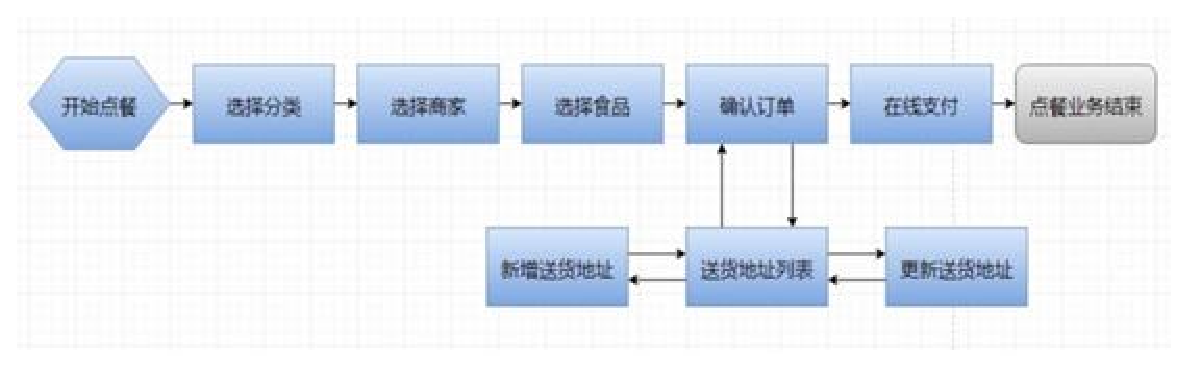
\includegraphics[width=0.8\textwidth]{progress}
\caption{点餐业务流程图}\label{fig:xml}
\vspace{\baselineskip}
\end{figure}
\begin{verbatim}
1.登录
实现方式:将输入匹配已经存在数据库user表中的userId和password,若匹配成功则登录用户。
实现接口:UserController/getUserByIdByPass

2.注册
实现方式:将注册新用户输入的信息存入数据库的user表中,向表中加一条新记录。
实现接口:UserController/saveUser

3.选择分类
实现方式:不同的分类代表着不同的orderTypeId,根据business表中属性orderTypeId查询所属business信息,返回business数组。
实现接口:BusinessController/listBusinessByOrderTypeId

4.选择商家
实现方式:将business对象封装起来,根据business表中的businessId查询business对象信息,最终返回business对象。
实现接口:BusinessController/getBusinessById

5.选择食品
功能1:呈现食品列表
实现方式:将food对象封装,在food表中businessId查询所属食品信息,最终返回food对象的数组。
实现接口:FoodController/listFoodByBusinessId

功能2:添加食品
实现方式:将食品信息、商家信息和用户信息向cart表中添加一条记录
实现接口:CartController/saveCart

功能3:在购物车中更改食品数量
实现方式:点击“+”号或“-”号,将cart表中的quantity的属性值加1或减1(值不为0)。
实现接口:CartController/updateCart

功能4: 移出购物车
实现方式:cart表中的quantity的属性值为0时,在cart表中根据userId、businessId、foodId删除该记录。
实现接口:CartController/removeCart

6.选择地址
功能1:新增地址
实现方式:将输入信息存入deliveryaddress表中,向表中添加一条记录。
实现接口:DeliveryAddressController/saveDeliveryAddress

功能2:更改地址信息
实现方式:根据daId更新送货地址的各属性值。
实现接口:DeliveryAddressController/updateDeliveryAddress

功能3:删除地址
实现方式:在deliveryaddress表中根据daId删除该daId对应的记录。
实现接口:DeliveryAddressController/removeDeliveryAddress

功能4:显示用户可选地址列表
实现方式:将deliveryAddress对象封装,在deliveryaddress表根据userId查询所属送货地址,返回deliveryAddress数组,再根据daId查询送货地址,返回deliveryAddress对象。
实现接口:DeliveryAddressController/listDeliveryAddressByUserId
DeliveryAddressController/getDeliveryAddressById

7.确认订单(在线支付)
实现方式:根据userId、businessId、orderTotal、daId向orders表中添加一条记录,并获取自动生成的orderId。然后根据userId、businessId从cart表中查询所有数据,批量添加到orderdetailet表中,然后根据用户编号、商家编号删除cart表中的数据。
实现接口:OrdersController/createOrders   
         CartController/removeCart

8.查询历史订单:
实现方式:将orders对象封装,在orders表中根据userId号查询此用户的所有订单信息,返回orders数组。根据orderId查询订单信息,包括所属商家信息,和此订单的所有订单明细信息。
实现接口:OrdersController/listOrdersByUserId  
         OrdersController/getOrdersById
\end{verbatim}


\section{SpringBoot后端设计}

\subsection{开发环境}

\begin{enumerate}
    \item 开发工具:SpringToolSuite、MySql、Navicat
    \item STS的jdk配置:jdk8
    \item Maven构建工具的配置: Maven3
    \item STS的文件编码配置:utf-8
\end{enumerate}

\subsection{架构模式}
基于Springboot+VUE-Cli的前后端分离工程

\begin{verbatim}
                用户层
                  | 
             Controller层
                  |
               Service层
                  |
                 Mapper层
                  |
             Database数据库
\end{verbatim}

\begin{enumerate}
\item Controller层:负责具体的业务模块流程的控制,在此层要调用service层的接口来控制业务流程,负责url映射,针对具体的业务流程,会有不同的控制器。
\item Service层:主要负责业务模块的应用逻辑应用设计,设计接口和其实现类,在Spring的配置文件中配置其实现的关联,这样我们就可以在应用中调用service接口来进行业务处理。service层的业务层具体要调用已经定义的dao层接口
\item Mapper层:即Dao层,主要负责数据持久层的工作,负责与数据库进行联络的一些任务都封装在此,需要设计接口及其实现类,直接对数据库进行操作(增删改查)。
\end{enumerate}

\subsection{功能及接口实现}
\begin{verbatim}
同Servlet 
    \end{verbatim}


	% !Mode:: "TeX:UTF-8"

\chapter{项目部署}

\section{JDBC项目部署}


\subsection {项目技术架构}
    \begin{itemize}
        \item JDK8
        \item JDBC
        \item MySql
    \end{itemize}

\subsection {开发工具}
    \begin{itemize}
        \item Intellij IDEA
        \item mysql
        \item navicat
    \end{itemize}

\subsection {安装部署指南}
\begin{enumerate}
    \item 安装 jdk、STS、MySql
    \item 在 mysql 数据库中创建数据库 elm\_admin,使用数据库脚本elm\_admin.sql 创建数据库和初始数据。
    \item 在 STS 中导入 javaSE 项目。
    \item 打开 com/neusoft/elm/util/DBUtil 修改数据库密码
\end{enumerate}

\section{前端项目部署}

\subsection{项目技术架构}
    \begin{itemize}
        \item HTML
        \item CSS
        \item JavaScript
    \end{itemize}

\subsection{开发工具}
    \begin{itemize}
        \item HBuilder
        \item Chrome浏览器
    \end{itemize}
    
\subsection{安装部署指南}
\begin{enumerate}
    \item 安装 hbuilder、chrome
    \item 将工程导入到 hbuilder 中
    \item 在 chrome 浏览器中运行 index.html 文件
    \item 在 chrome 浏览器中使用 Toggle device toolbar 模拟手机浏览
\end{enumerate}

\section{Servlet项目部署}

\subsection{项目前端技术架构}
    \begin{itemize}
        \item VUE-CLI
    \end{itemize}

\subsection{项目后端技术架构}
    \begin{itemize}
        \item JDK 1.8
        \item Servlet
        \item Tomcat 8.5
        \item MySql
    \end{itemize}
    
\subsection{开发工具}
    \begin{itemize}
        \item 前端项目:HBuilder
        \item 后端项目:Spring-tool-suite
        \item Tomcat 8.5
        \item MySql
        \item Navicat
    \end{itemize}

\subsection {安装部署指南}
\begin{itemize}
    \item {后端项目部署}
        \begin{enumerate}
            \item 安装 jdk、STS、Tomcat、MySql
            \item 在 mysql 数据库中创建数据库 elm,使用数据库脚本 elm.sql 创建数据
            库和初始数据。
            \item 在 STS 中导入 elm 项目,并部署到 Tomcat 中。
            \item 打开 com/neusoft/elm/util/DBUtil 修改数据库密码
            \item 启动 Tomcat
        \end{enumerate}
    \item {前端项目部署}
        \begin{enumerate}
            \item 安装 Node.js、安装 Vue-Cli
            \item 首先将前端工程导入到 hbuilder 中
            \item 切换到项目路径下,使用 npm 安装依赖: npm install, 安装成功后,在
            项目文件夹下出现 node\_modules 文件夹,里面是项目依赖。
            \item 启动项目 npm run serve
            \item 在浏览器中输入网址 http://localhost:8081,进入首页
        \end{enumerate}
\end{itemize}

\section{SpringBoot项目部署}

\subsection{项目前端技术架构}
    \begin{itemize}
        \item VUE-CLI
    \end{itemize}

\subsection{项目后端技术架构}
    \begin{itemize}
        \item JDK 1.8
        \item SpringBoot
        \item MyBatis
        \item MySql
        \item Maven
    \end{itemize}
    
\subsection{开发工具}
    \begin{itemize}
        \item 前端项目:HBuilder
        \item 后端项目:Spring-tool-suite
        \item MySql
        \item Navicat
        \item Maven
    \end{itemize}

\subsection {安装部署指南}
\begin{itemize}
    \item {后端项目部署}
        \begin{enumerate}
            \item 安装 jdk、Maven、STS、MySql
            \item 在 mysql 数据库中创建数据库 elm,使用数据库脚本 elm.sql 创建数据库和初始数据。
            \item 在 STS 中导入 elmboot 的 Maven 项目。
            \item 打开 SpringBoot 配置文件 application.properties 修改数据库密码。
            \item 运行 ElmbootApplication
        \end{enumerate}
    \item {前端项目部署}
        \begin{enumerate}
            \item 安装 Node.js、安装 Vue-Cli
            \item 首先将前端工程导入到 hbuilder 中
            \item 切换到项目路径下,使用 npm 安装依赖: npm install, 安装成功后,在
            项目文件夹下出现 node\_modules 文件夹,里面是项目依赖。
            \item 启动项目 npm run serve
            \item 在浏览器中输入网址 http://localhost:8081,进入首页
        \end{enumerate}
\end{itemize}

	% !Mode:: "TeX:UTF-8"

\chapter{项目测试}

\section{前端测试}

根据UI效果图进行UI测试
\begin{enumerate}
\item 观察APP的用户界面(如菜单、对话框、窗口和其它可规控件)是否符合UI稿
\item 不同的连接页面之间导航链接是否有效,是否跳转是否正确
\item 输入框说明文字的内容与产品需求一致
\item 某页无数据时、断网时、有网但接口异常时的状态页是否和UI一致
\end{enumerate}

\section{接口测试}
\begin{enumerate}
\item Get,post发送和返回是否请求正常
\item 查看请求参数和返回参数结果是否正常
\end{enumerate}
(测试接口工具:postman)

\section{功能测试}
业务功能流程如图\ref{fig:prog}所示
\begin{figure}[htbp]
    \centering
    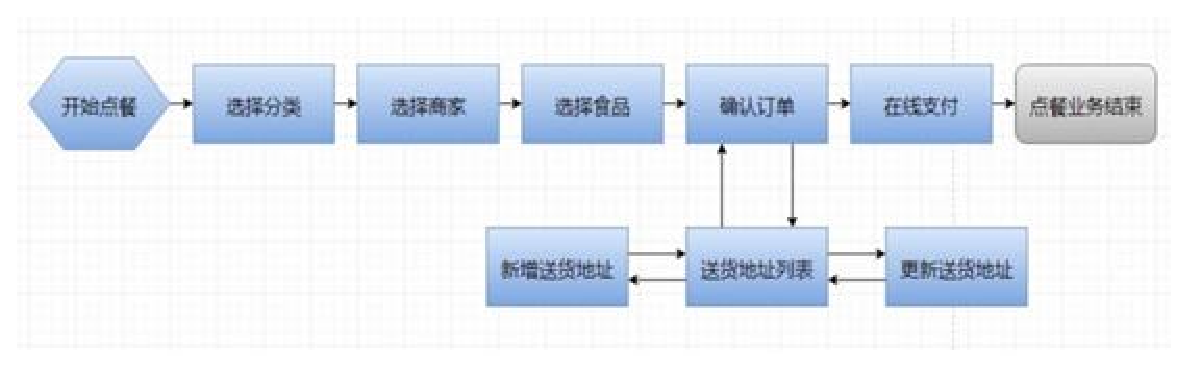
\includegraphics[width=0.8\textwidth]{progress}
    \caption{点餐业务流程图}\label{fig:prog}
    \vspace{\baselineskip}
    \end{figure}

    
\begin{verbatim}
    功能测试在前后端连接之后,主要按照点餐业务流程图的功能依次进行测试,依据编写的功能测试用例进行软件功能的测试。通过观察实行操作后页面的显示,提示框的弹出以及数据库内容的改变来判断功能是否完成。
    
\end{verbatim}
	% !Mode:: "TeX:UTF-8"

\chapter{项目特色}
\begin{enumerate}
\item
\begin{figure}[htbp]
    \centering
    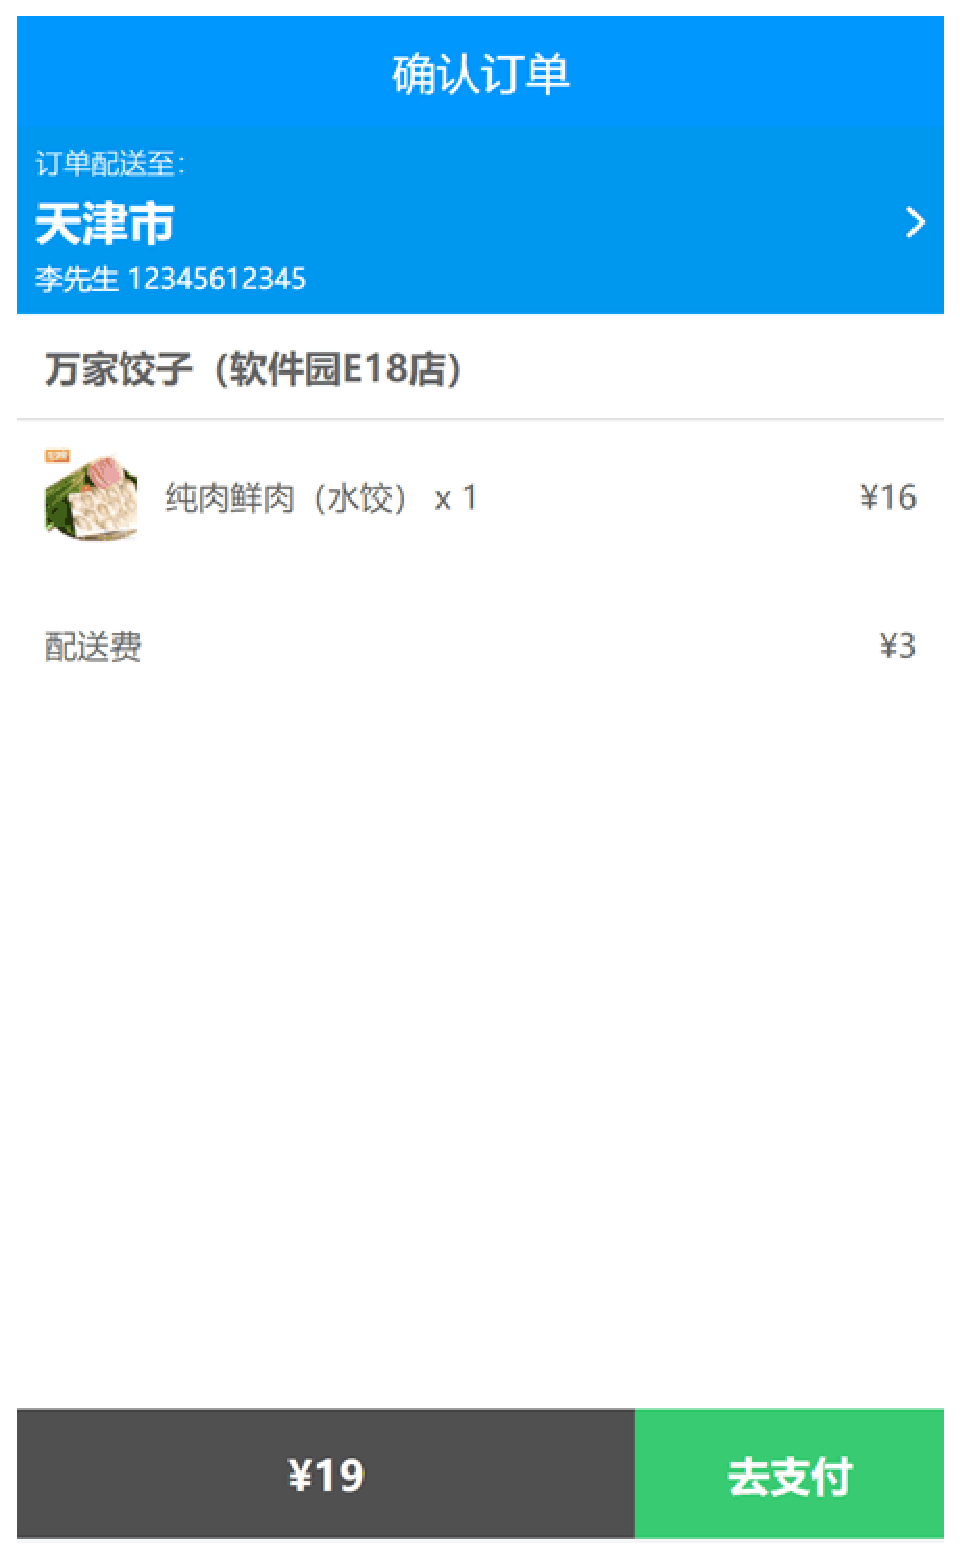
\includegraphics[width=0.6\textwidth]{order}
    \caption{确认订单}\label{fig:ord}
    \vspace{\baselineskip}
    \end{figure}

\begin{verbatim}
确认订单页面中,在选择地址时发现该项目与实际不符合的情况:当切换地址时,该项目会将地址改变,而地址下的姓名和电话仍为userName和userId,实际情况应为deliveryaddress表中的contactName和contactTel.
因此在此处做出修改:
当该用户的deliveryaddress为空时,则此处的姓名和电话为userName和userId,当该用户的deliveryaddress不为空时,此处的姓名和电话为contactName和contactTel。
\end{verbatim}    

\item
\begin{figure}[htbp]
    \centering
    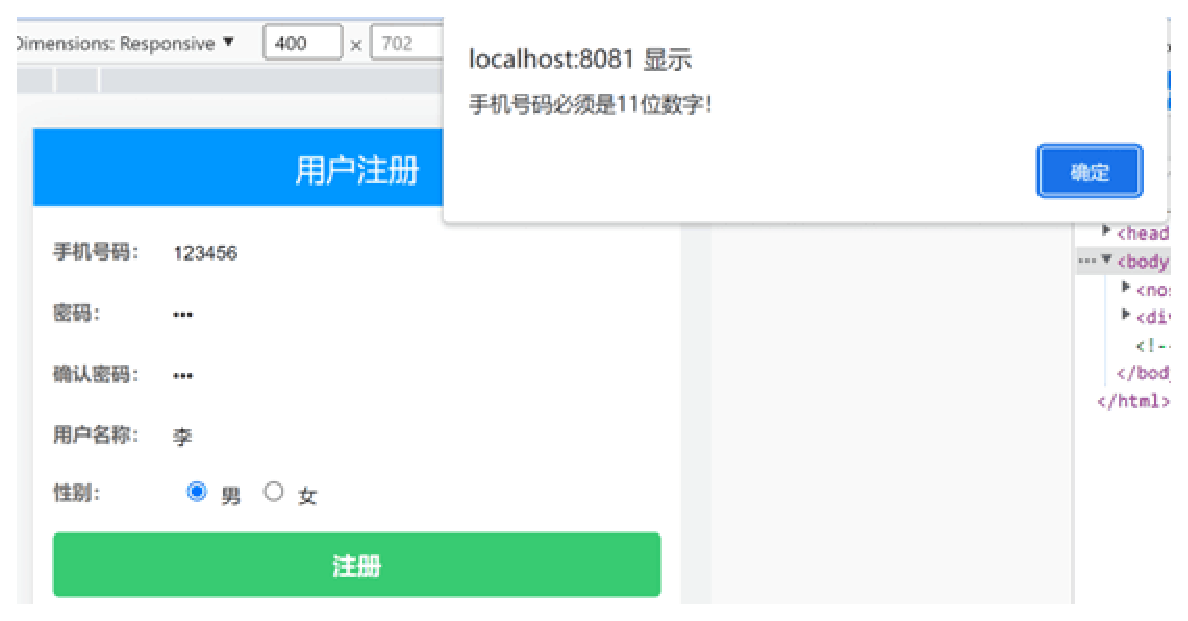
\includegraphics[width=0.8\textwidth]{11}
    \caption{注册页面}\label{fig:xml}
    \vspace{\baselineskip}
    \end{figure}

\begin{verbatim}
用户注册页面中,由于正确的手机号码应为11位数字。
因此在此处做出修改:
当输入的手机号码不为11位时,弹出提示框“手机号码必须是11位数字”    
\end{verbatim}

\begin{figure}[htbp]
\centering
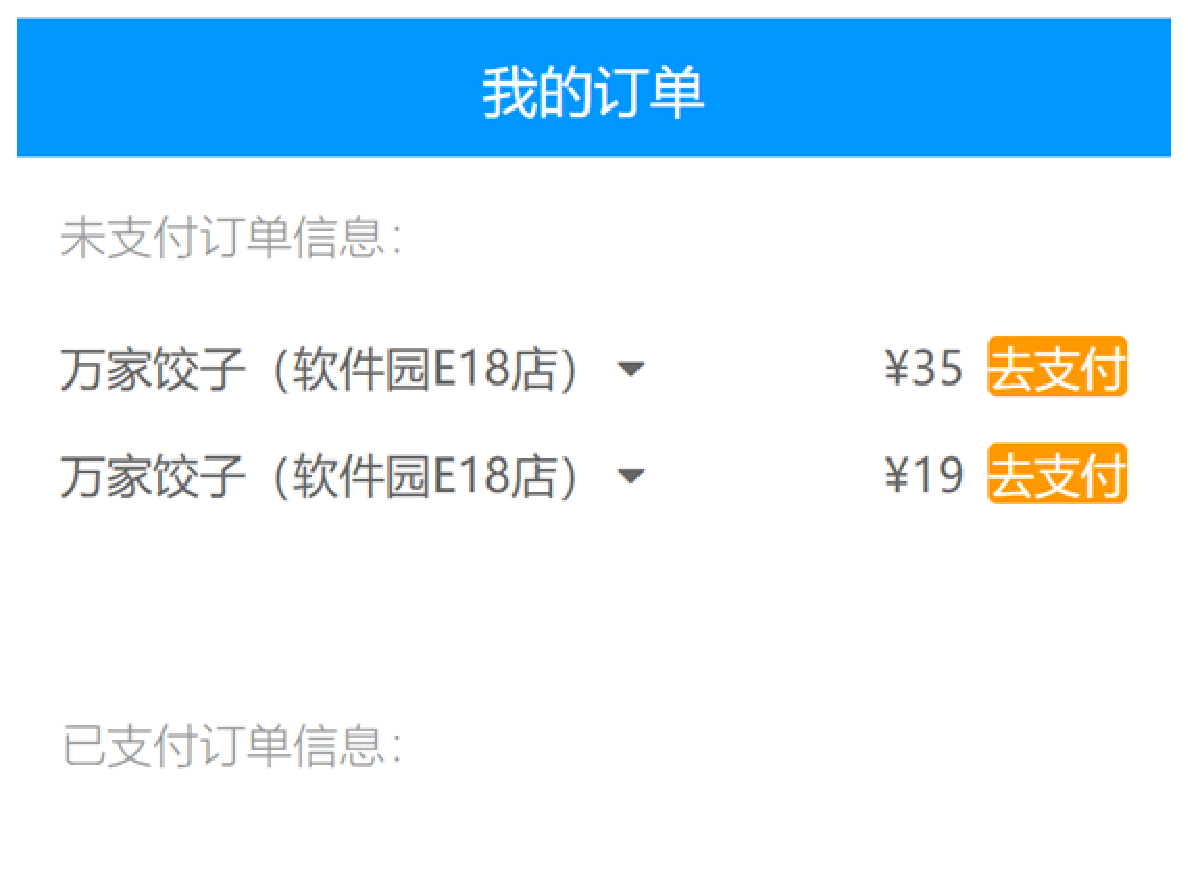
\includegraphics[width=0.8\textwidth]{pay}
\caption{我的订单}\label{fig:xml}
\vspace{\baselineskip}
\end{figure}

\item
\begin{verbatim}
在我的订单页面,由于此页面去支付未设置功能。
因此在此处做出修改:
点击去支付按钮,跳转到支付页面。
      
\end{verbatim}


\end{enumerate}
	% !Mode:: "TeX:UTF-8"

\chapter{附录}

\section{异构计算实验截图}
\begin{verbatim}
1.闫佑诚实验截图
uid:u165347
\end{verbatim}
\begin{figure}[htbp]
    \centering
    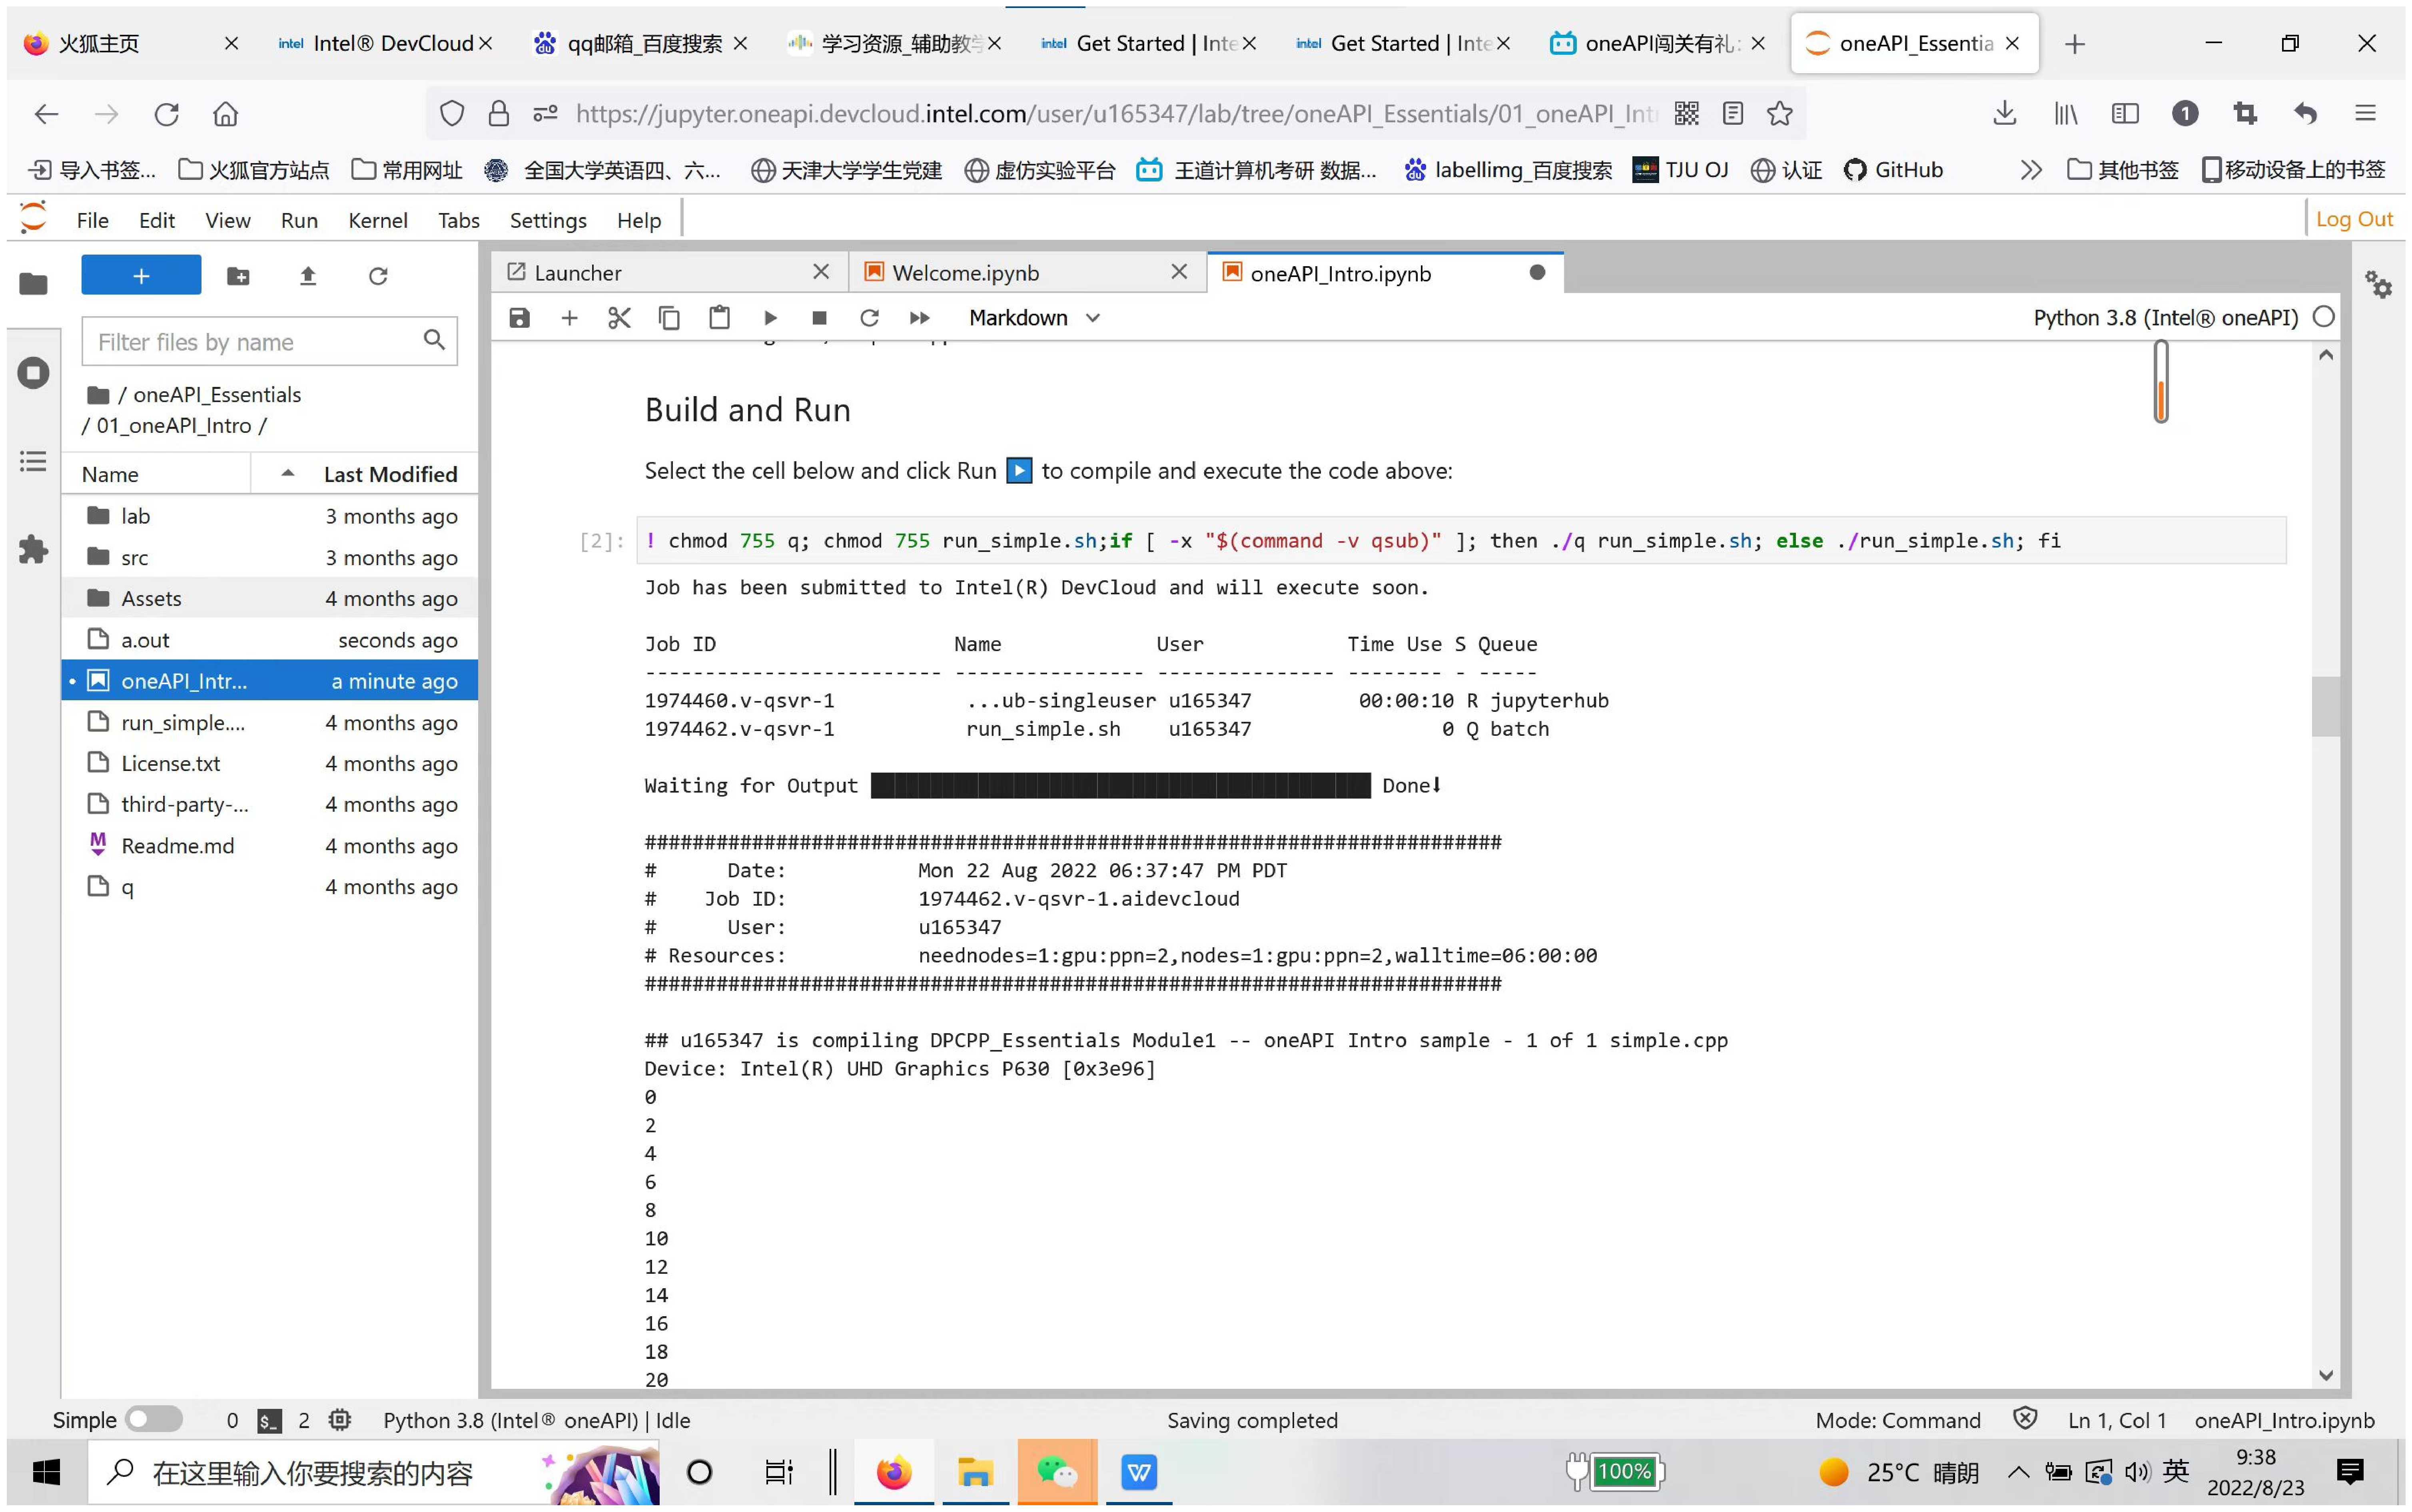
\includegraphics[width=1\textwidth]{uid1}
    \caption{异构计算实验截图1}\label{fig:UID1}
    \vspace{\baselineskip}
    \end{figure}
    
\begin{verbatim}
2.胡亿权实验截图
uid:u165346
\end{verbatim}
\begin{figure}[htbp]
    \centering
    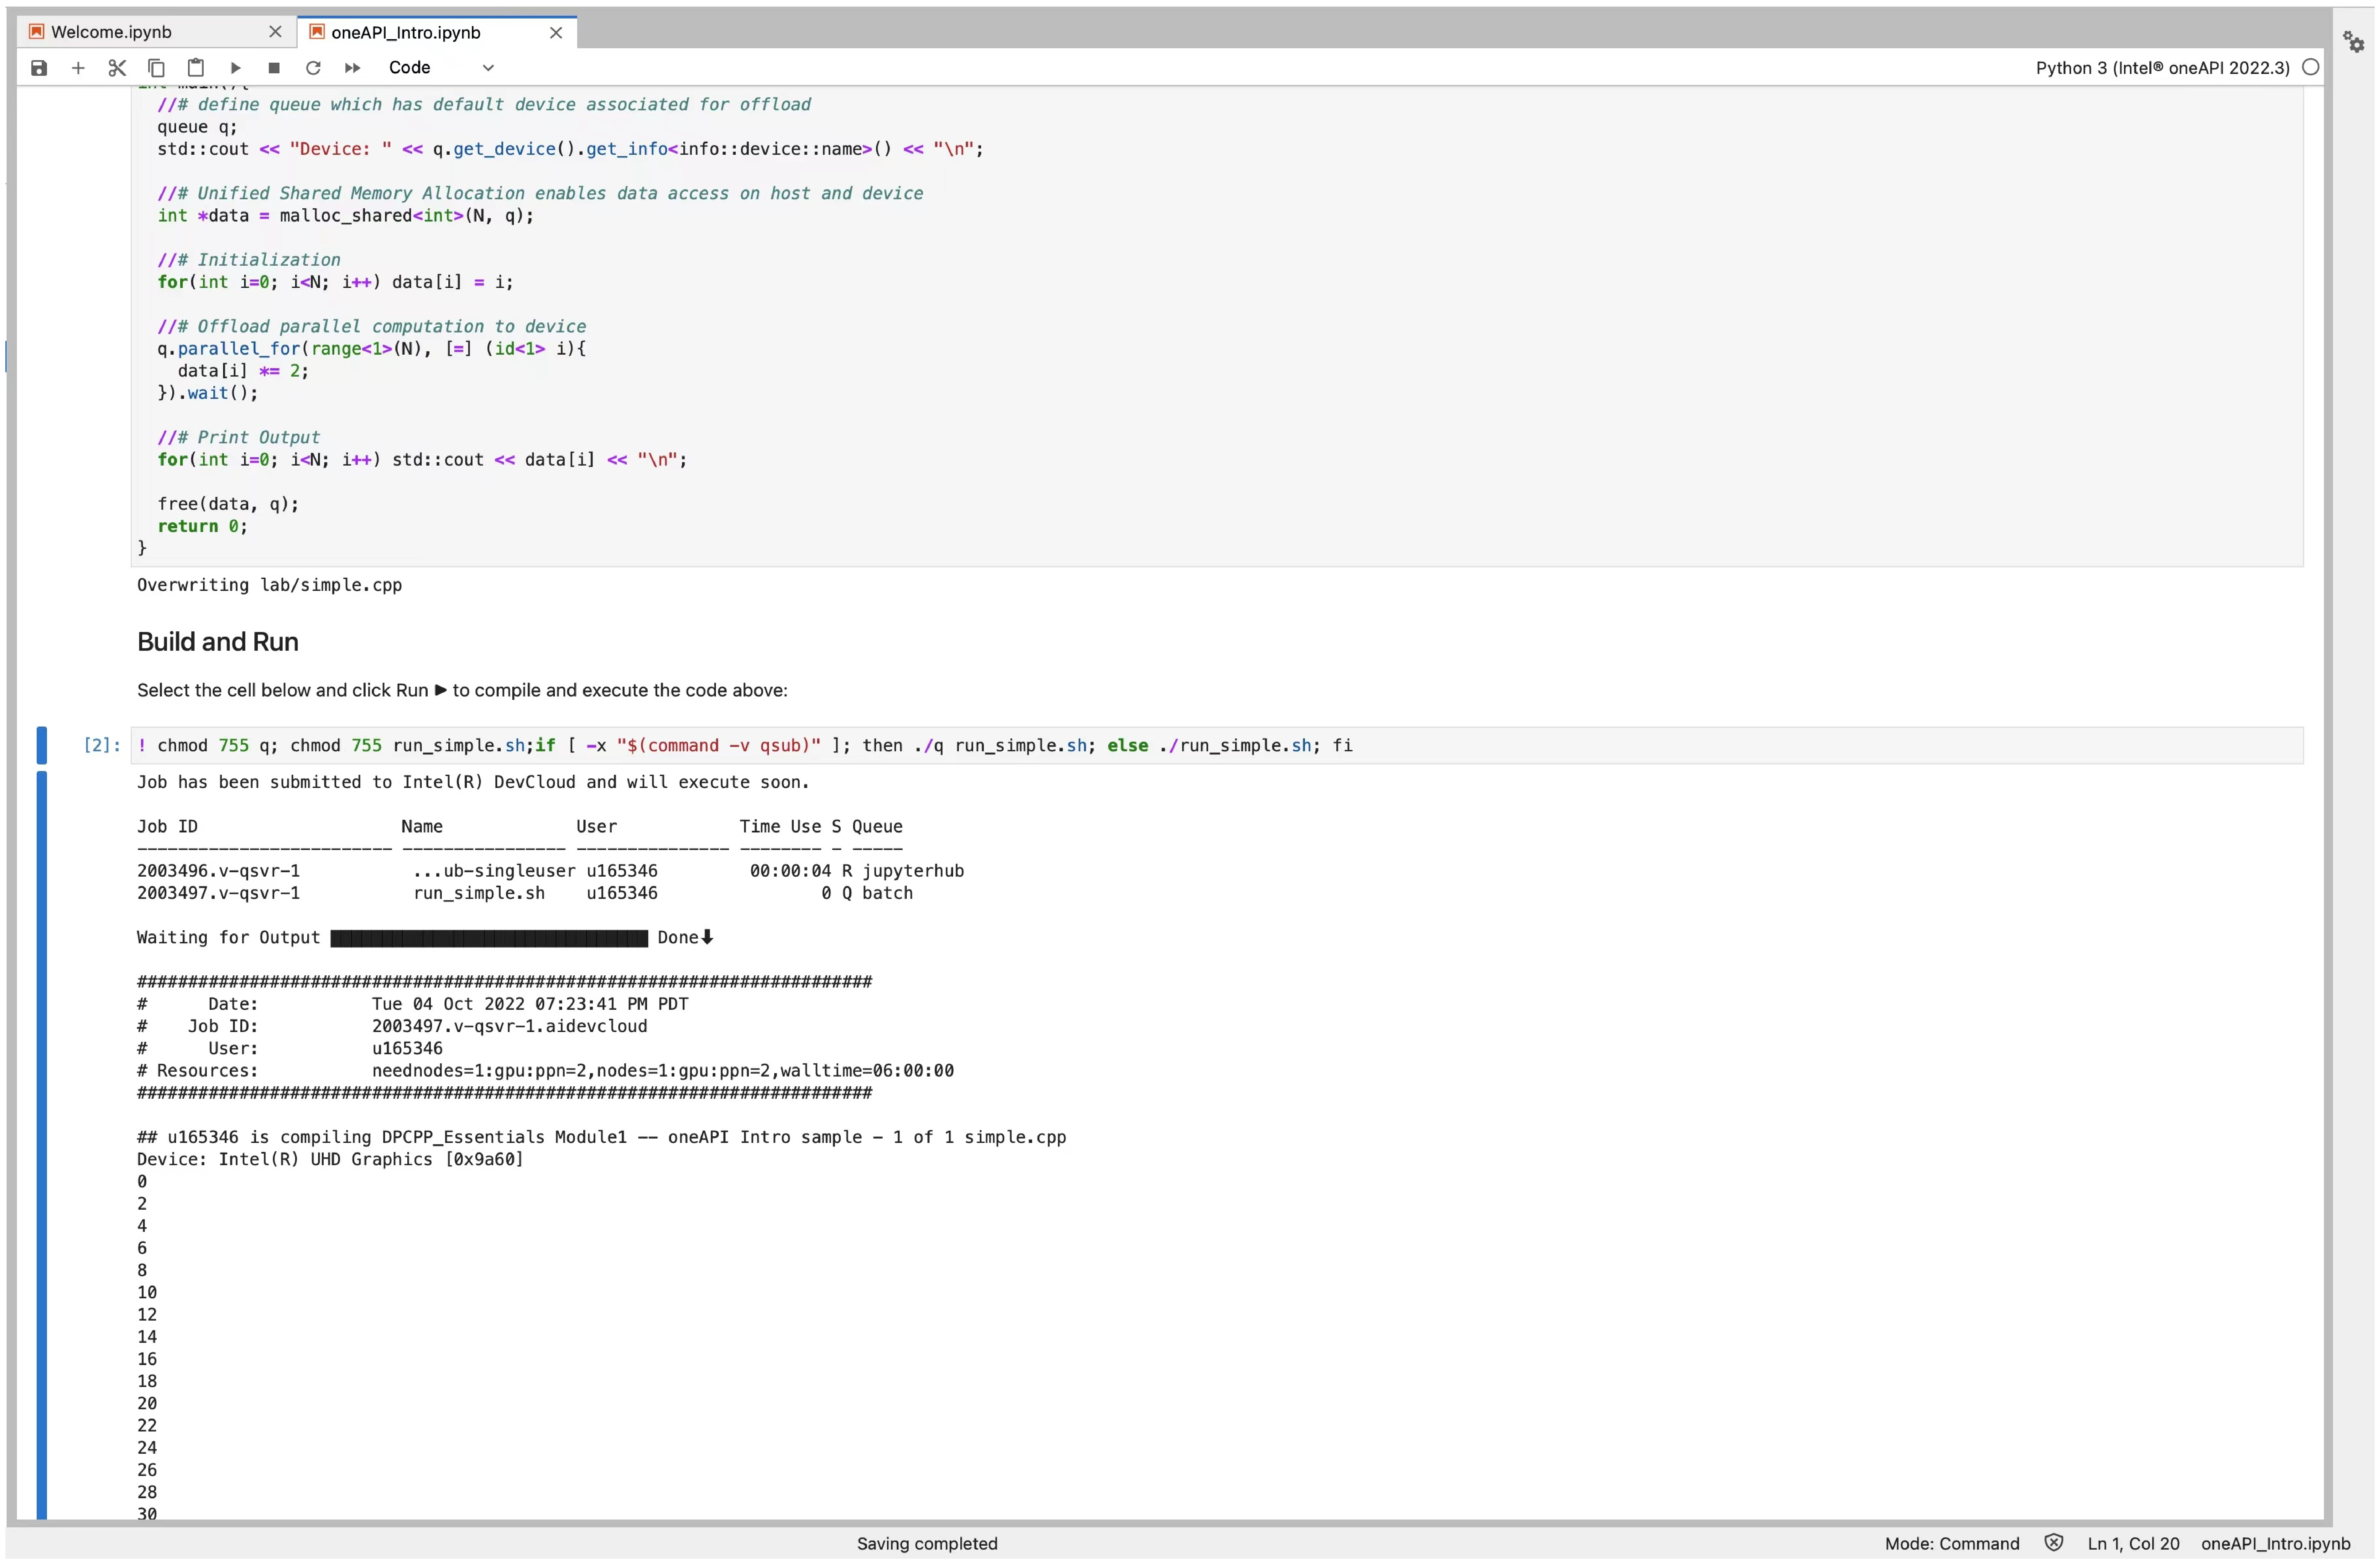
\includegraphics[width=1\textwidth]{uidhyq}
    \caption{异构计算实验截图2}\label{fig:UID2}
    \vspace{\baselineskip}
    \end{figure}


\begin{verbatim}
3.韦唯佳实验截图
uid:u172160
\end{verbatim}
\begin{figure}[htbp]
\centering
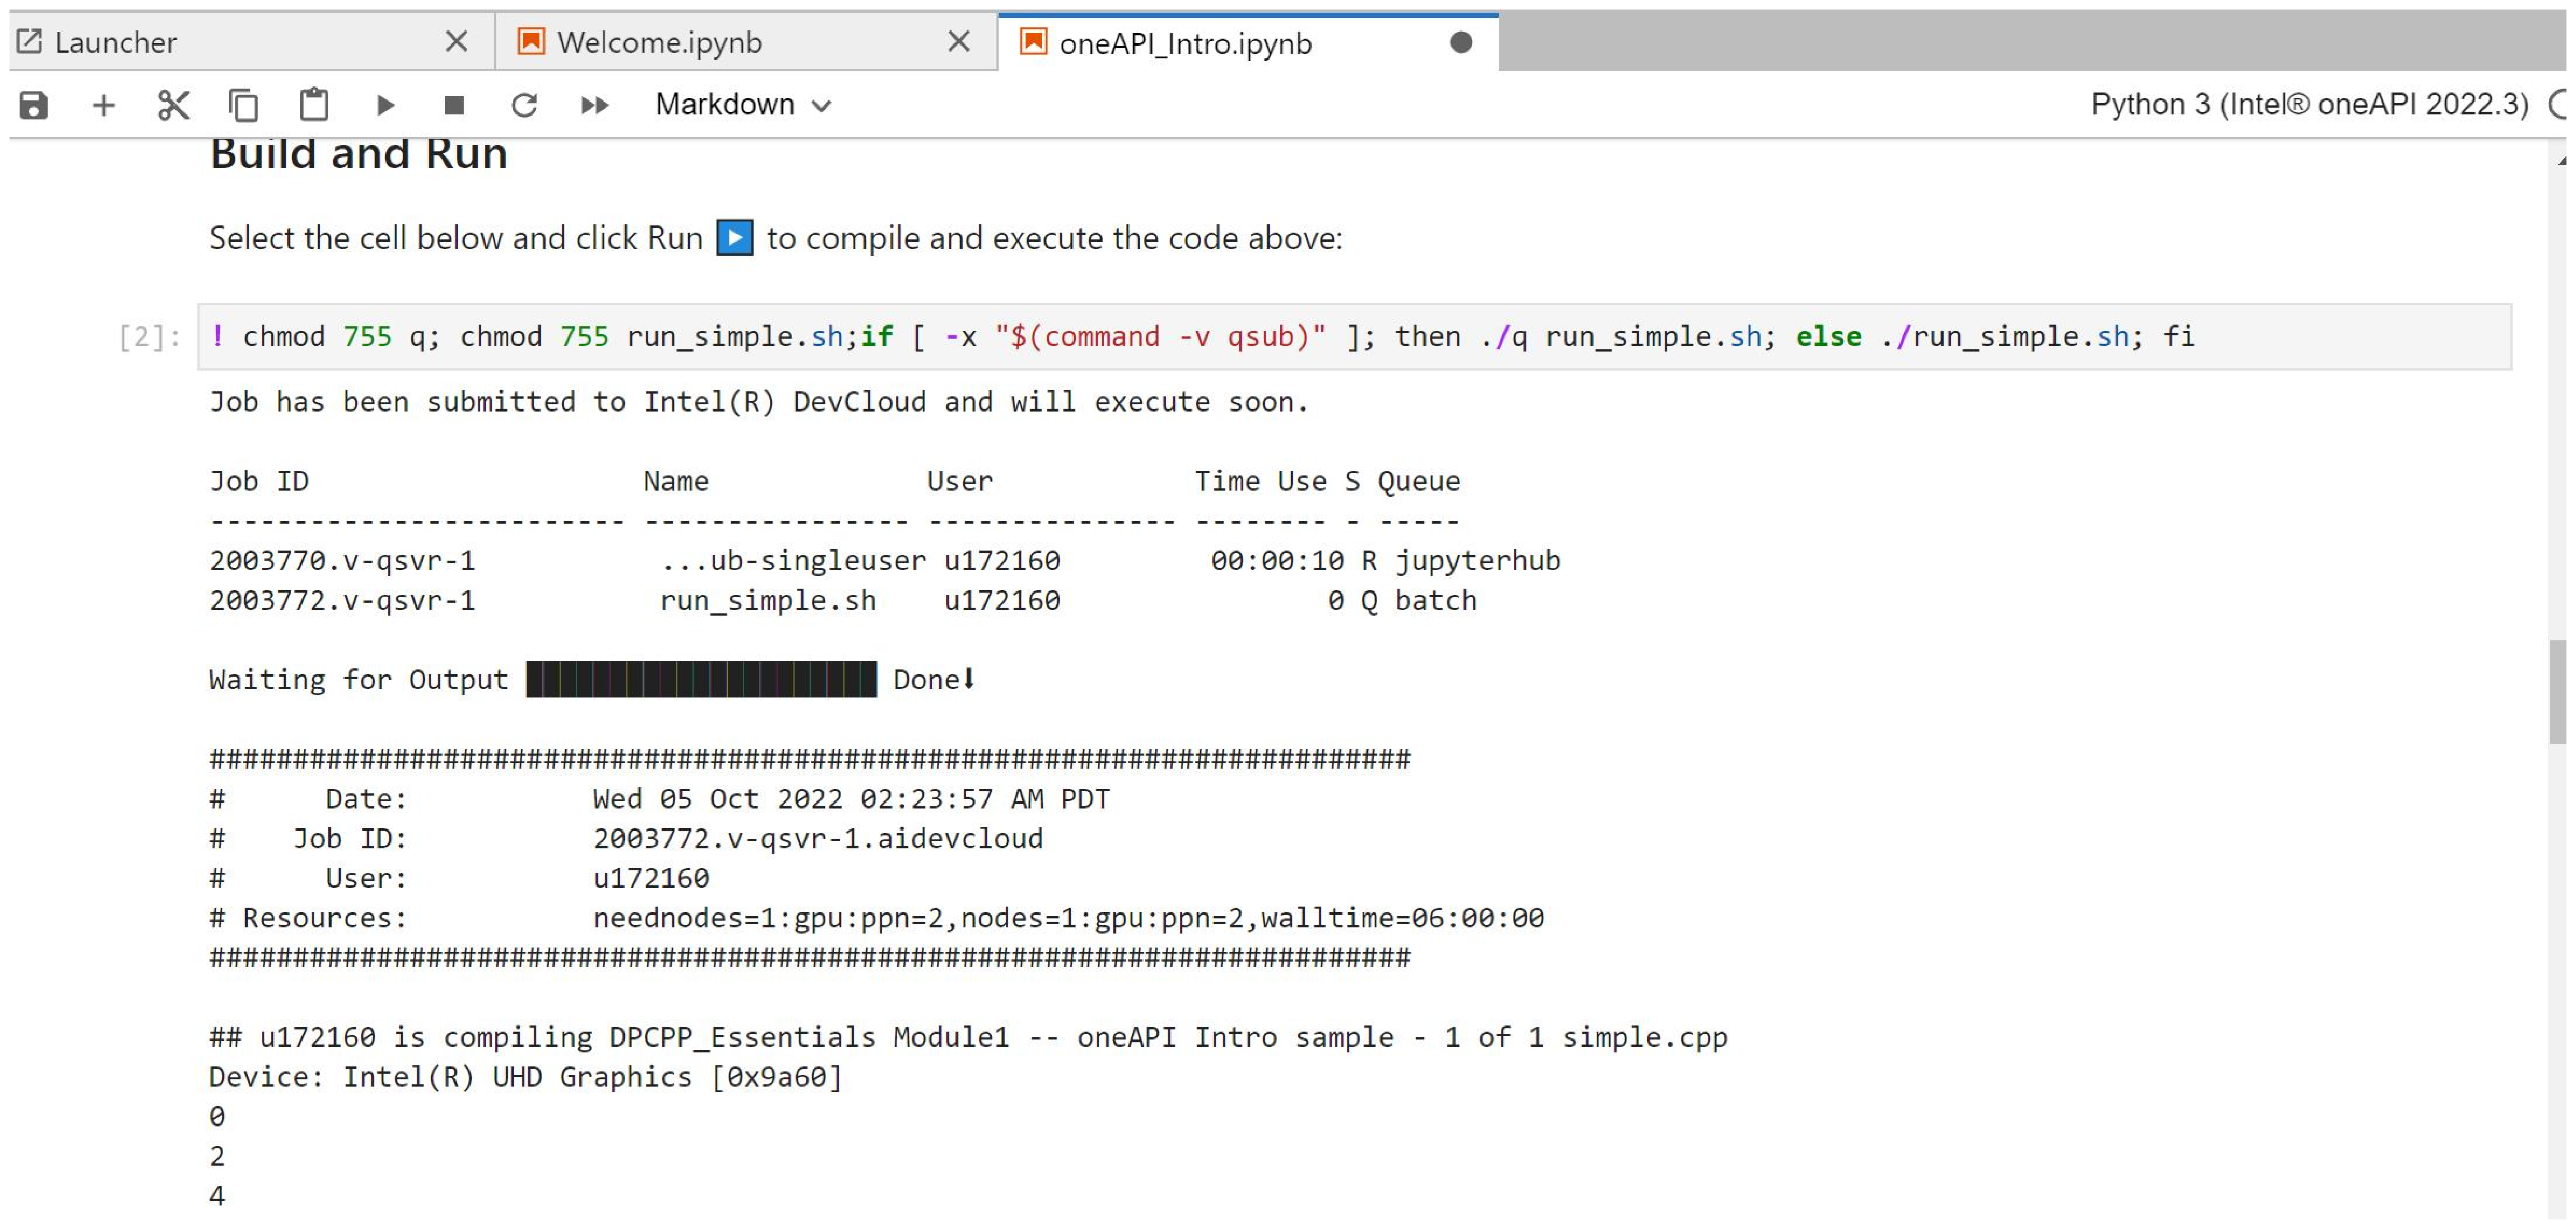
\includegraphics[width=1\textwidth]{uidwwj}
\caption{异构计算实验截图3}\label{fig:UID3}
\vspace{\baselineskip}
\end{figure}



	% \clearpage

\end{CJK*}                                     % 结束中文字体使用
\end{document}                                 % 结束全文
